\section{General Principles}
\begin{tcolorbox}[title=Data Validation]
\textbf{Dilbert:} I didn't have any accurate numbers, so I just made up this one. Studies have shown that accurate numbers aren't any more useful that the ones you make up. \\ 
\textbf{Pointy-Haired Boss:} How many studies showed that? \\ 
\textbf{Dilbert:} [\textit{beat}] Eighty-seven.\\[-0.6cm]
\begin{flushright}
-- Scott Adams, \newhref{http://dilbert.com/strip/2008-05-08}{Dilbert}, 8 May 2008
\end{flushright}
\end{tcolorbox}
\noindent
\subsection{Approaches to Data Cleaning}
There are two main \textbf{philosophical} approaches to data cleaning and validation: 
\begin{itemize}[noitemsep]
\item \textbf{methodical}, and  
\item \textbf{narrative}.
\end{itemize}
 The \textbf{methodical} approach consists in running through a \textbf{check list} of potential issues and flagging those that apply to the data.
\par The \textbf{narrative} approach, on the other hand, consists in \textbf{exploring} the dataset while searching for unlikely or irregular patterns. 
\newl
Which approach the consultant/analyst opts to follow depends on a number of factors, not least of which is the client's needs and views  on the matter -- it is important  to discuss this point with the clients.
\subsection{Pros and Cons}
The methodical approach focuses on  \textbf{syntax}; the check-list is typically \textbf{context-independent}, which means that it (or a subset) can be reused from one project to another, which makes data analysis pipelines \textbf{easy to implement} and \textbf{automate}. In the same vein, common errors are \textbf{easily identified}.\par  On the flip side, the check list may be quite extensive and the entire process may prove \textbf{time-consuming}.\par The biggest disadvantage of this approach is that it makes it difficult to identify \textbf{new types of errors}.\newl
The narrative approach focuses on \textbf{semantics}; even false starts may simultaneously produce \textbf{data understanding} prior to switching to a more mechanical approach.\par It is easy, however, to miss important sources of errors and invalid observations when the datasets have a \textbf{large number of features}. \par There is an additional downside: \textbf{domain expertise}, coupled with the narrative approach,  may bias the process by neglecting ``uninteresting'' areas of the dataset.
\subsection{Tools and Methods} A non-exhaustive list of common data issues can be found in the \textit{Data Cleaning Bingo Card} (see Table~\ref{fig:bingo}); other possibilities obviously exist. \newl Other methods include 
\begin{itemize}[noitemsep]
\item \textbf{visualizations} -- which may help easily identify observations that need to be further examined;
\item \textbf{data summaries} -- \# of missing observations; 5-pt summary, mean, standard deviation, skew, kurtosis, for numerical variables; distribution tables for categorical variables; 
\item \textbf{$n$-way tables} -- counts for joint distributions of categorical variables;
\item \textbf{small multiples} -- tables/visualizations indexed along categorical variables, and
\item \textbf{preliminary data analyses} -- which may provide ``huh, that's odd...'' realizations.   
\end{itemize}
It is important to note that there is nothing wrong with running a number of analyses to flush out data issues, but remember to label your initial forays as \textbf{preliminary} analyses. From the client's perspective, repeated analyses may create a sense of unease and distrust, even if they form a crucial part of the analytical process (doing so will also facilitate invoicing, if that is part of your concern). 
\begin{center}
    \rule{0.5\linewidth}{.4pt}
\end{center}
In our (admittedly biased and incomplete) experience, \begin{itemize}[noitemsep]
\item \textbf{computer scientists} and \textbf{programmers} tend to naturally favour the methodical approach, while \item \textbf{mathematicians} and \textbf{statisticians} tend to naturally favour the narrative approach,
\end{itemize}
although we have met plenty of individuals with unexpected backgrounds in both camps. This is not the place for identity politics: quantitative consultants and analysts need to be comfortable with \textbf{both} approaches. 
\newl As an example, the narrative approach is akin to working out a crossword puzzle with a pen and accepting to put down potentially erroneous answers once in a while to try to open up the grid (what artificial intelligence researchers call the ``exploration'' approach). \par The mechanical approach, on the other hand, is similar to working out the puzzle with a pencil and a dictionary, only putting down answers when their correctness is guaranteed (the ``exploitation'' approach of artificial intelligence). \newl More puzzles get solved when using the first approach, but mistakes tend to be spectacular. Not as many puzzles get solved the second way, but the trade-off is that that it leads to fewer mistakes. 

\begin{table*}[!t]
\centering
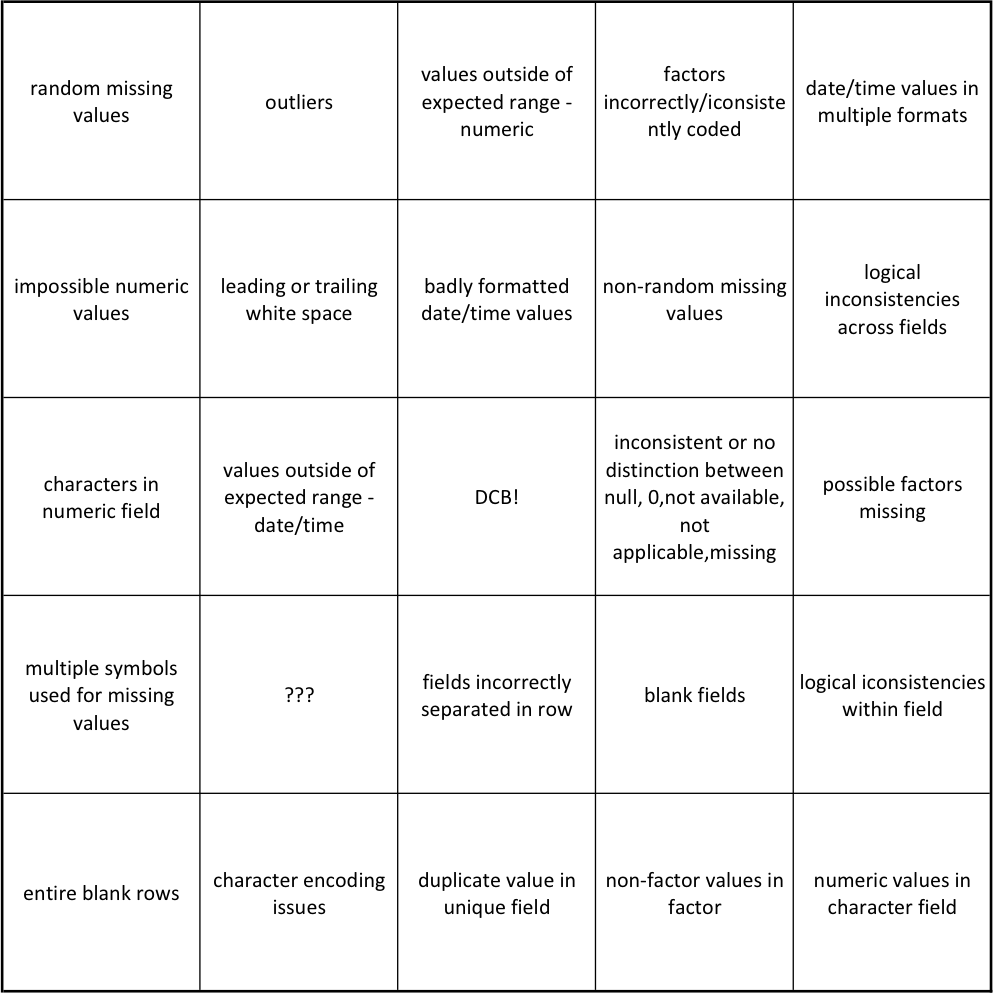
\includegraphics[width=0.75\textwidth]{Images/bingo.png}
\caption{\small Data cleaning bingo card [personal communication, J.Shellinck].} \label{fig:bingo}\hrule
\end{table*}
